
\begin{center}
\Huge
	Cosinusrelationerne
\end{center}

\section*{Cosinusrelationerne}
\stepcounter{section}

I tilfældet at vi kender to sider og den mellemstående vinkel, så kan vi bruge \textit{cosinusrelationerne} til at bestemme den sidste sidelængde. Dette var også netop de betingelser, vi havde for at kunne bestemme arealet for en trekant. 

\begin{setn}[Cosinusrelationerne]
	\label{setn:cosinusrelationerne}
	For vilkårlige trekanter $\triangle ABC$ som den på Figur \ref{fig:vilkårlig} har vi følgende sammenhæng
	mellem sidelængderne og vinklerne i trekanten.
	\begin{align}
	\label{eq:cos1}
	\begin{split}
		c^2 &= a^2 + b^2 - 2ab\cos(\angle C),  \\
		b^2 &= a^2 + c^2 - 2ac\cos(\angle B), \\
		a^2 &= b^2 + c^2 - 2bc\cos(\angle A).
	\end{split}
	\end{align}
\end{setn}

Som det var tilfældet med sinusrelationerne, kan vi også omskrive cosinusrelationerne, så det er nemmere at finde vinklen, hvis vi kun kender sidelængder. Så lyder cosinusrelationerne

\begin{align}
	\label{eq:cos2}
	\begin{split}
	\cos(\angle C) &= \frac{a^2 + b^2 - c^2}{2ab},\\
	\cos(\angle B) &= \frac{a^2 + c^2 - b^2}{2ac},\\
	\cos(\angle A) &= \frac{b^2 + c^2 - a^2}{2bc}.
	\end{split}
\end{align}

\begin{figure}[H]
	\centering
	\begin{tikzpicture}
		\draw[color = olive, thick] (0,0) -- (5,0) node[midway, anchor = north] {$b$};
		\draw[color = olive, thick] (0,0) -- (4,3) node[midway, anchor = south east] {$c$};
		\draw[color = olive, thick] (5,0) -- (4,3) node[midway, anchor = west] {$a$};
		\node[color = olive, anchor = east] at (0,0) {$A$};
		\node[color = olive, anchor = west] at (5,0) {$C$};
		\node[color = olive, anchor = south] at (4,3) {$B$};
	\end{tikzpicture}
	\caption{Vilkårlig trekant $\triangle ABC$}
	\label{fig:vilkårlig}
\end{figure}

Vi betragter selvfølgelig også et eksempel for at se, hvordan vi kan anvende cosinusrelationerne. 
\begin{exa}
	En trekant $\triangle ABC$ er givet ved følgende.
	\begin{center}
		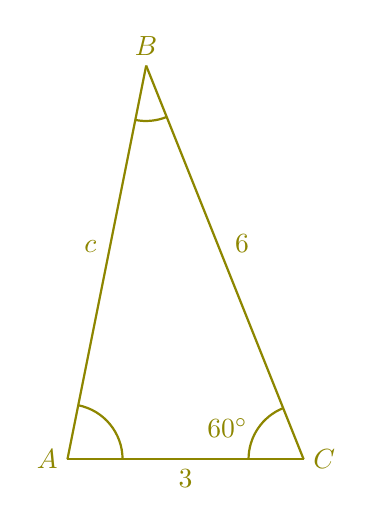
\begin{tikzpicture}
		%A
		\pgfmathsetmacro{\ax}{0}
		\pgfmathsetmacro{\ay}{0}
		%B
		\pgfmathsetmacro{\bx}{1}
		\pgfmathsetmacro{\by}{5}
		%C
		\pgfmathsetmacro{\cx}{3}
		\pgfmathsetmacro{\cy}{0}
		%arc radius
		\pgfmathsetmacro{\arclen}{0.7}
		%c
		\draw[color = olive, thick] (\ax,\ay) -- (\bx,\by) node[midway, anchor = south east] {$c$};
		%b
		\draw[color = olive, thick] (\ax,\ay) -- (\cx,\cy) node[midway, anchor = north] {$3$};
		%a
		\draw[color = olive, thick] (\bx,\by) -- (\cx,\cy) node[midway, anchor = south west] {$6$};
	%	Vinkel A		
		\draw[color = olive, thick] (\arclen,0) arc (0:78.68:\arclen) 
		node[midway, anchor = west] {};
	%	Vinkel B
		\draw[color = olive, thick] (0.86,4.31) arc (180 + 78.69:180 + 78.69 + 33.11:\arclen)
		 node[midway, anchor = south] {};
	%	Vinkel C
		\draw[color = olive, thick] (\cx - \arclen,0) arc (180:180 - 68.20:\arclen)
		 node[midway, anchor = east] {$60^\circ$};
		 %Nodes
		 \node[color = olive, anchor = east] at (\ax,\ay) {$A$};
		 \node[color = olive, anchor = south] at (\bx,\by) {$B$};
		 \node[color = olive, anchor = west] at (\cx,\cy) {$C$};
		\end{tikzpicture}
	\end{center}
	Vi ved, at $a = 6$, $b = 3$ og $\angle C = 60^\circ$. Først aflæses $\cos(60^\circ) = 0.5$ i 
	Tabel \ref{tab:cossintan}, og efterfølgende indsættes dette i den første ligning i
	 Sætning \ref{setn:cosinusrelationerne}, hvor vi får
	\begin{align*}
		c^2 &= a^2 + b^2 -2ab\cos(\angle C) \\
		&= 6^2 + 3^2 - 2\cdot 6\cdot 3 \cdot 0.5 \\
		&= 27.
	\end{align*}
	Vi kan nu finde længden af $c$ som
	\begin{align*}
		c = \sqrt{27} = \sqrt{9\cdot 3} = \sqrt{9}\sqrt{3} = 3\sqrt{3}.
	\end{align*}
	Dette giver os altså $c = 3\sqrt{3}$. 
\end{exa} 

Hvis vi skal bestemme sidelængder med cosinusrelationerne, så er tilsvarende til sinusrelationerne nemmest at bruge \eqref{eq:cos1}, og skal vi bestemme vinkler med cosinusrelationerne, er det nemmest at bruge \eqref{eq:cos2}.

\newpage


\begin{table}[H]
	\centering
	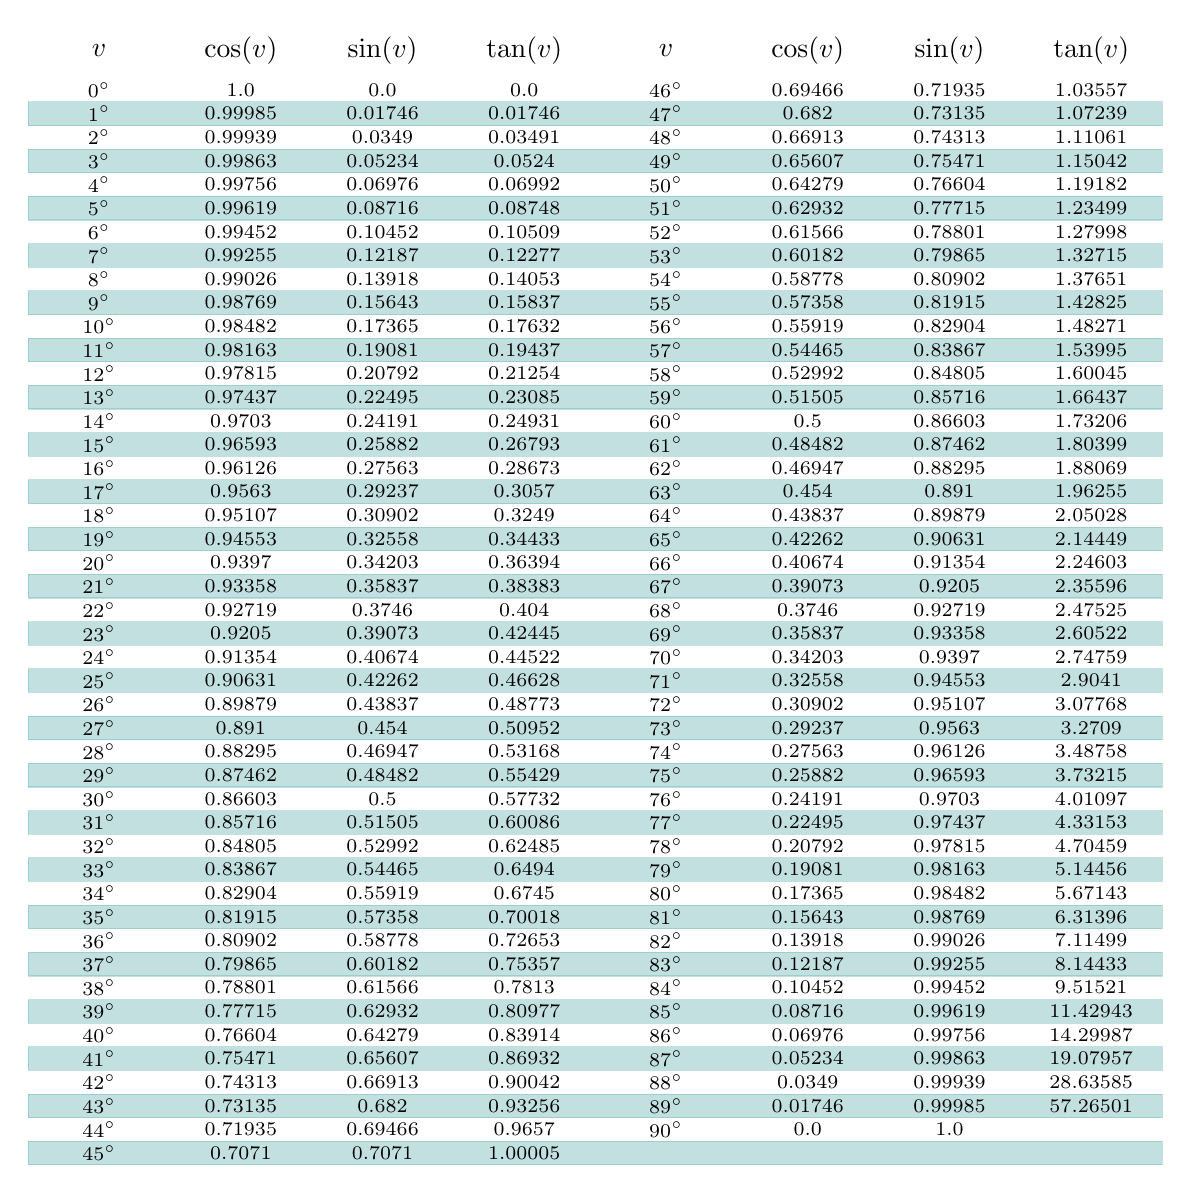
\begin{tikzpicture}
	\node at (0,0) {$v$};
	\node at (2*0.9,0) {$\cos(v)$};
	\node at (4*0.9,0) {$\sin(v)$};
	\node at (6*0.9,0) {$\tan(v)$};
	\node at (8*0.9,0) {$v$};
	\node at (10*0.9,0) {$\cos(v)$};
	\node at (12*0.9,0) {$\sin(v)$};
	\node at (14*0.9,0) {$\tan(v)$};
	\scriptsize
	%Colors
	\foreach \i in {0,...,22}{
		\filldraw[color = teal!60, opacity = 0.4] (-0.9,-0.5-0.3+0.15-\i*0.3*2) rectangle
		 (14*0.9 + 0.9,-0.5-0.3-0.15-\i*0.3*2);
	}
	\foreach \i in {0,...,45}{
		%Macros for evaluating
		\pgfmathsetmacro{\cval}{cos(\i)}
		\pgfmathsetmacro{\sval}{sin(\i)}
		\pgfmathsetmacro{\tval}{tan(\i)}
		%First columns of values
		\node at (0,-0.5-\i*0.3) {$\i^{\circ}$};
		\node at (2*0.9,-0.5-\i*0.3) { \cval };
		\node at (4*0.9,-0.5-\i*0.3) { \sval };
		\node at (6*0.9,-0.5-\i*0.3) { \tval };
	}
	\foreach \i in {46,...,89}{
		%Macros
		\pgfmathsetmacro{\cval}{cos(\i)}
		\pgfmathsetmacro{\sval}{sin(\i)}
		\pgfmathsetmacro{\tval}{tan(\i)}
		%Second column
		\node at (8*0.9,-0.5-\i*0.3 + 46*0.3) {$\i^{\circ}$};
		\node at (10*0.9,-0.5-\i*0.3 + 46*0.3) { \cval };
		\node at (12*0.9,-0.5-\i*0.3 + 46*0.3) { \sval };
		\node at (14*0.9,-0.5-\i*0.3 + 46*0.3) { \tval };
	}
		\pgfmathsetmacro{\cval}{cos(90)}
		\pgfmathsetmacro{\sval}{sin(90)}
		\node at (8*0.9,-0.5-90*0.3 + 46*0.3) {$90^{\circ}$};
		\node at (10*0.9,-0.5-90*0.3 + 46*0.3) { \cval };
		\node at (12*0.9,-0.5-90*0.3 + 46*0.3) { \sval };
	\end{tikzpicture}
	\caption{Tabel over udvalgte værdier for $\cos$, $\sin$ og $\tan$.}
	\label{tab:cossintan}
\end{table}

\newpage

\subsection*{Opgave 1}
Til de følgende to delopgaver skal du bruge Tabel \ref{tab:cossintan}, hvor du afrunder til to decimaler.
\begin{enumerate}[label=\roman*)]
	\item Bestem sidelængden $a$ i den første trekant.
	\item Bestem sidelængden $b$ i den anden trekant. 
\begin{center}
	\begin{minipage}{0.45\textwidth}
		\centering
		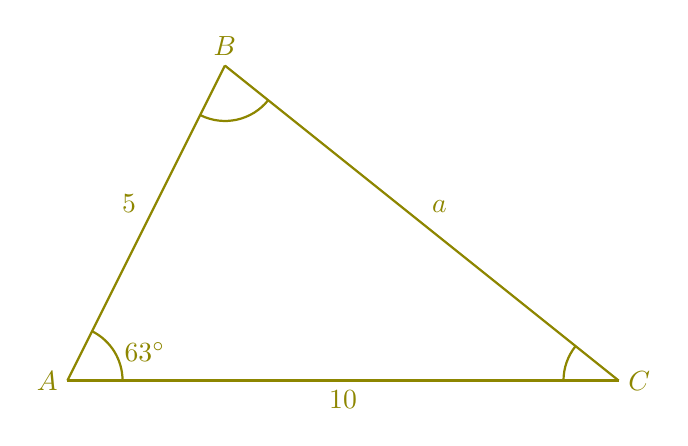
\begin{tikzpicture}
		%A
		\pgfmathsetmacro{\ax}{0}
		\pgfmathsetmacro{\ay}{0}
		%B
		\pgfmathsetmacro{\bx}{2}
		\pgfmathsetmacro{\by}{4}
		%C
		\pgfmathsetmacro{\cx}{7}
		\pgfmathsetmacro{\cy}{0}
		%arc radius
		\pgfmathsetmacro{\arclen}{0.7}
		%c
		\draw[color = olive, thick] (\ax,\ay) -- (\bx,\by) node[midway, anchor = south east] {$5$};
		%b
		\draw[color = olive, thick] (\ax,\ay) -- (\cx,\cy) node[midway, anchor = north] {$10$};
		%a
		\draw[color = olive, thick] (\bx,\by) -- (\cx,\cy) node[midway, anchor = south west] {$a$};
	%	Vinkel A		
		\draw[color = olive, thick] (\arclen,0) arc (0:63.43:\arclen) 
		node[midway, anchor = west] {$63^\circ$};
	%	Vinkel B
		\draw[color = olive, thick] (1.69,3.37) arc (180 + 63.53:180 + 63.43 + 77.91:\arclen)
		 node[midway, anchor = south] {};
	%	Vinkel C
		\draw[color = olive, thick] (\cx - \arclen,0) arc (180:180 - 38.66:\arclen)
		 node[midway, anchor = east] {};
		 %Nodes
		 \node[color = olive, anchor = east] at (\ax,\ay) {$A$};
		 \node[color = olive, anchor = south] at (\bx,\by) {$B$};
		 \node[color = olive, anchor = west] at (\cx,\cy) {$C$};
		\end{tikzpicture}
	\end{minipage}
	\begin{minipage}{0.45\textwidth}
		\centering
		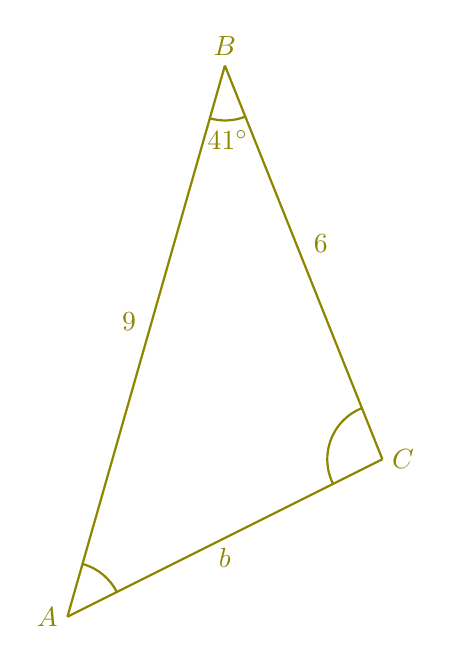
\begin{tikzpicture}
		%A
		\pgfmathsetmacro{\ax}{0}
		\pgfmathsetmacro{\ay}{0}
		%B
		\pgfmathsetmacro{\bx}{2}
		\pgfmathsetmacro{\by}{7}
		%C
		\pgfmathsetmacro{\cx}{4}
		\pgfmathsetmacro{\cy}{2}
		%arc radius
		\pgfmathsetmacro{\arclen}{0.7}
		%c
		\draw[color = olive, thick] (\ax,\ay) -- (\bx,\by) node[midway, anchor = south east] {$9$};
		%b
		\draw[color = olive, thick] (\ax,\ay) -- (\cx,\cy) node[midway, anchor = north] {$b$};
		%a
		\draw[color = olive, thick] (\bx,\by) -- (\cx,\cy) node[midway, anchor = south west] {$6$};
	%	Vinkel A		
		\draw[color = olive, thick] (0.63,0.31) arc (26.57:47.49+26.57:\arclen) 
		node[midway, anchor = south west] {};
	%	Vinkel B
		\draw[color = olive, thick] (1.81,6.33) arc (180 + 74.05:180+74.05+37.75:\arclen)
		 node[midway, anchor = north] {$41^{\circ}$};
	%	Vinkel C
		\draw[color = olive, thick] (3.74,2.65) arc (111.8:111.8+94.76:\arclen)
		 node[midway, anchor = east] {};
		 %Nodes
		 \node[color = olive, anchor = east] at (\ax,\ay) {$A$};
		 \node[color = olive, anchor = south] at (\bx,\by) {$B$};
		 \node[color = olive, anchor = west] at (\cx,\cy) {$C$};
		\end{tikzpicture}
	\end{minipage}
\end{center}
\end{enumerate}

\newpage

\subsection*{Opgave 2}
Til de følgende to delopgaver skal du bruge Tabel \ref{tab:cossintan}, hvor du afrunder til to decimaler.
\begin{enumerate}[label=\roman*)]
	\item Bestem sidelængden $c$ i den første trekant.
	\item Bestem sidelængden $b$ i den anden trekant. 
\end{enumerate}
\begin{center}
	\begin{minipage}{0.45\textwidth}
		\centering
		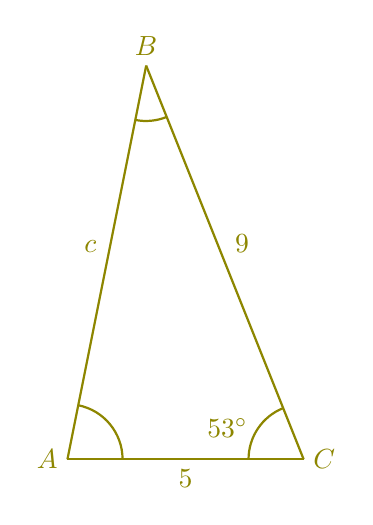
\begin{tikzpicture}
		%A
		\pgfmathsetmacro{\ax}{0}
		\pgfmathsetmacro{\ay}{0}
		%B
		\pgfmathsetmacro{\bx}{1}
		\pgfmathsetmacro{\by}{5}
		%C
		\pgfmathsetmacro{\cx}{3}
		\pgfmathsetmacro{\cy}{0}
		%arc radius
		\pgfmathsetmacro{\arclen}{0.7}
		%c
		\draw[color = olive, thick] (\ax,\ay) -- (\bx,\by) node[midway, anchor = south east] {$c$};
		%b
		\draw[color = olive, thick] (\ax,\ay) -- (\cx,\cy) node[midway, anchor = north] {$5$};
		%a
		\draw[color = olive, thick] (\bx,\by) -- (\cx,\cy) node[midway, anchor = south west] {$9$};
	%	Vinkel A		
		\draw[color = olive, thick] (\arclen,0) arc (0:78.68:\arclen) 
		node[midway, anchor = west] {};
	%	Vinkel B
		\draw[color = olive, thick] (0.86,4.31) arc (180 + 78.69:180 + 78.69 + 33.11:\arclen)
		 node[midway, anchor = south] {};
	%	Vinkel C
		\draw[color = olive, thick] (\cx - \arclen,0) arc (180:180 - 68.20:\arclen)
		 node[midway, anchor = east] {$53^\circ$};
		 %Nodes
		 \node[color = olive, anchor = east] at (\ax,\ay) {$A$};
		 \node[color = olive, anchor = south] at (\bx,\by) {$B$};
		 \node[color = olive, anchor = west] at (\cx,\cy) {$C$};
		\end{tikzpicture}
	\end{minipage}
		\begin{minipage}{0.45\textwidth}
		\centering
		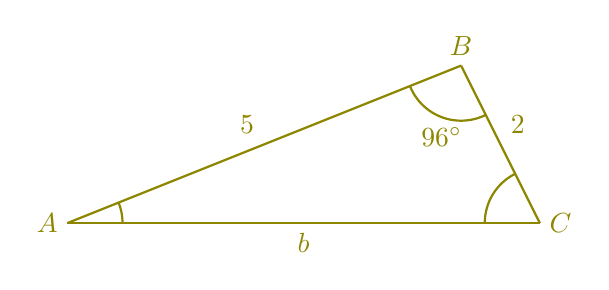
\begin{tikzpicture}
		%A
		\pgfmathsetmacro{\ax}{0}
		\pgfmathsetmacro{\ay}{0}
		%B
		\pgfmathsetmacro{\bx}{5}
		\pgfmathsetmacro{\by}{2}
		%C
		\pgfmathsetmacro{\cx}{6}
		\pgfmathsetmacro{\cy}{0}
		%arc radius
		\pgfmathsetmacro{\arclen}{0.7}
		%c
		\draw[color = olive, thick] (\ax,\ay) -- (\bx,\by) node[midway, anchor = south east] {$5$};
		%b
		\draw[color = olive, thick] (\ax,\ay) -- (\cx,\cy) node[midway, anchor = north] {$b$};
		%a
		\draw[color = olive, thick] (\bx,\by) -- (\cx,\cy) node[midway, anchor = south west] {$2$};
	%	Vinkel A		
		\draw[color = olive, thick] (\arclen,0) arc (0:21.8:\arclen) 
		node[midway, anchor = west] {};
	%	Vinkel B
		\draw[color = olive, thick] (4.35,1.74) arc (180 + 21.8:180 + 21.8 + 94.76:\arclen)
		 node[midway, anchor = north] {$96^\circ$};
	%	Vinkel C
		\draw[color = olive, thick] (\cx - \arclen,0) arc (180:180 - 63.43:\arclen)
		 node[midway, anchor = east] {};
		 %Nodes
		 \node[color = olive, anchor = east] at (\ax,\ay) {$A$};
		 \node[color = olive, anchor = south] at (\bx,\by) {$B$};
		 \node[color = olive, anchor = west] at (\cx,\cy) {$C$};
		\end{tikzpicture}
	\end{minipage}
\end{center}

\newpage

\subsection*{Opgave 3}
Til de følgende to delopgaver skal du bruge Tabel \ref{tab:cossintan}, hvor du afrunder til to decimaler.
\begin{enumerate}[label=\roman*)]
	\item Bestem vinklen $\angle B$ i den første trekant.
	\item Bestem vinklen $\angle B$ i den anden trekant.  
\end{enumerate}
\begin{center}
		\begin{minipage}{0.45\textwidth}
		\centering
		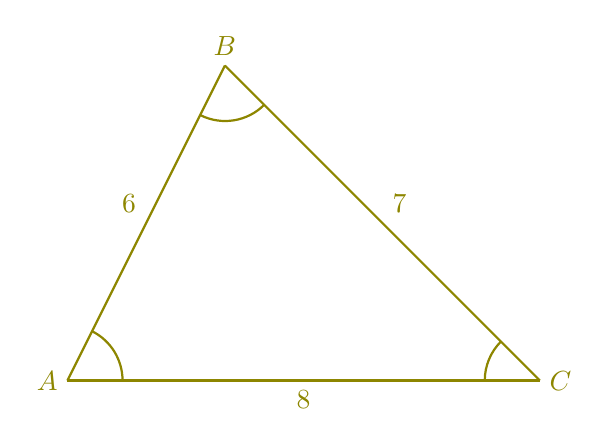
\begin{tikzpicture}
		%A
		\pgfmathsetmacro{\ax}{0}
		\pgfmathsetmacro{\ay}{0}
		%B
		\pgfmathsetmacro{\bx}{2}
		\pgfmathsetmacro{\by}{4}
		%C
		\pgfmathsetmacro{\cx}{6}
		\pgfmathsetmacro{\cy}{0}
		%arc radius
		\pgfmathsetmacro{\arclen}{0.7}
		%c
		\draw[color = olive, thick] (\ax,\ay) -- (\bx,\by) node[midway, anchor = south east] {$6$};
		%b
		\draw[color = olive, thick] (\ax,\ay) -- (\cx,\cy) node[midway, anchor = north] {$8$};
		%a
		\draw[color = olive, thick] (\bx,\by) -- (\cx,\cy) node[midway, anchor = south west] {$7$};
	%	Vinkel A		
		\draw[color = olive, thick] (\ax + \arclen,0) arc (0:63.43:\arclen) 
		node[midway, anchor = west] {};
	%	Vinkel B
		\draw[color = olive, thick] (1.69,3.37) arc (180 + 63.43:180 + 63.43 + 71.57:\arclen)
		 node[midway, anchor = south east] {};
	%	Vinkel C
		\draw[color = olive, thick] (\cx - \arclen,0) arc (180:180 - 45:\arclen)
		 node[midway, anchor = east] {};
		 %Nodes
		 \node[color = olive, anchor = east] at (\ax,\ay) {$A$};
		 \node[color = olive, anchor = south] at (\bx,\by) {$B$};
		 \node[color = olive, anchor = west] at (\cx,\cy) {$C$};
		\end{tikzpicture}
	\end{minipage}
	\begin{minipage}{0.45\textwidth}
		\centering
		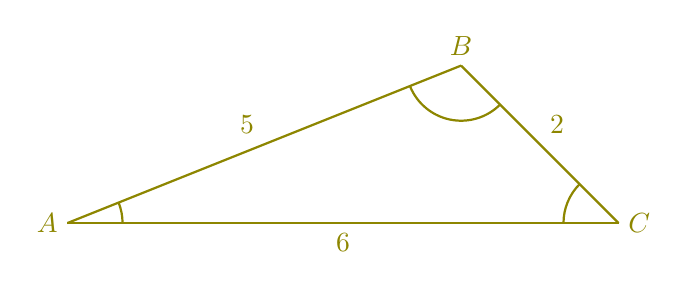
\begin{tikzpicture}
		%A
		\pgfmathsetmacro{\ax}{0}
		\pgfmathsetmacro{\ay}{0}
		%B
		\pgfmathsetmacro{\bx}{5}
		\pgfmathsetmacro{\by}{2}
		%C
		\pgfmathsetmacro{\cx}{7}
		\pgfmathsetmacro{\cy}{0}
		%arc radius
		\pgfmathsetmacro{\arclen}{0.7}
		%c
		\draw[color = olive, thick] (\ax,\ay) -- (\bx,\by) node[midway, anchor = south east] {$5$};
		%b
		\draw[color = olive, thick] (\ax,\ay) -- (\cx,\cy) node[midway, anchor = north] {$6$};
		%a
		\draw[color = olive, thick] (\bx,\by) -- (\cx,\cy) node[midway, anchor = south west] {$2$};
	%	Vinkel A		
		\draw[color = olive, thick] (\arclen,0) arc (0:21.8:\arclen) 
		node[midway, anchor = west] {};
	%	Vinkel B
		\draw[color = olive, thick] (4.35,1.74) arc (180 + 21.8:180 + 21.8 + 113.2:\arclen)
		 node[midway, anchor = north east] {};
	%	Vinkel C
		\draw[color = olive, thick] (\cx - \arclen,0) arc (180:180 - 45:\arclen)
		 node[midway, anchor = east] {};
		 %Nodes
		 \node[color = olive, anchor = east] at (\ax,\ay) {$A$};
		 \node[color = olive, anchor = south] at (\bx,\by) {$B$};
		 \node[color = olive, anchor = west] at (\cx,\cy) {$C$};
		\end{tikzpicture}
	\end{minipage}
\end{center}

\newpage

\subsection*{Opgave 4}
Til de følgende to delopgaver skal du bruge Tabel \ref{tab:cossintan}, hvor du afrunder til to decimaler.
\begin{enumerate}[label=\roman*)]
	\item Bestem vinklen $\angle C$ i den første trekant.
	\item Bestem vinklen $\angle A$ i den anden trekant. 
\end{enumerate}
\begin{center}
	\begin{minipage}{0.45\textwidth}
		\centering
		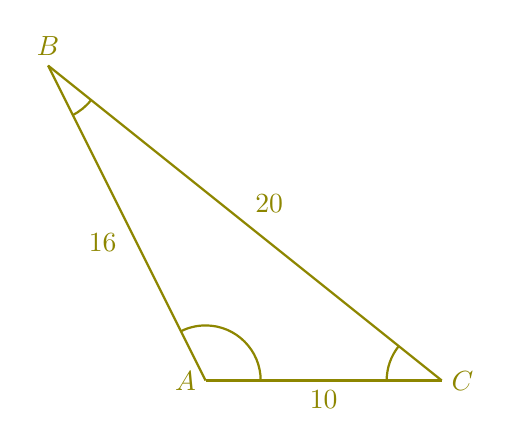
\begin{tikzpicture}
		%A
		\pgfmathsetmacro{\ax}{2}
		\pgfmathsetmacro{\ay}{0}
		%B
		\pgfmathsetmacro{\bx}{0}
		\pgfmathsetmacro{\by}{4}
		%C
		\pgfmathsetmacro{\cx}{5}
		\pgfmathsetmacro{\cy}{0}
		%arc radius
		\pgfmathsetmacro{\arclen}{0.7}
		%c
		\draw[color = olive, thick] (\ax,\ay) -- (\bx,\by) node[midway, anchor = north east] {$16$};
		%b
		\draw[color = olive, thick] (\ax,\ay) -- (\cx,\cy) node[midway, anchor = north] {$10$};
		%a
		\draw[color = olive, thick] (\bx,\by) -- (\cx,\cy) node[midway, anchor = south west] {$20$};
	%	Vinkel A		
		\draw[color = olive, thick] (\ax + \arclen,0) arc (0:116.57:\arclen) 
		node[midway, anchor = west] {};
	%	Vinkel B
		\draw[color = olive, thick] (0.31,3.37) arc (180 + 116.57:180 + 116.57 + 24.78:\arclen)
		 node[midway, anchor = south east] {};
	%	Vinkel C
		\draw[color = olive, thick] (\cx - \arclen,0) arc (180:180 - 38.66:\arclen)
		 node[midway, anchor = east] {};
		 %Nodes
		 \node[color = olive, anchor = east] at (\ax,\ay) {$A$};
		 \node[color = olive, anchor = south] at (\bx,\by) {$B$};
		 \node[color = olive, anchor = west] at (\cx,\cy) {$C$};
		\end{tikzpicture}
	\end{minipage}
	\begin{minipage}{0.45\textwidth}
		\centering
		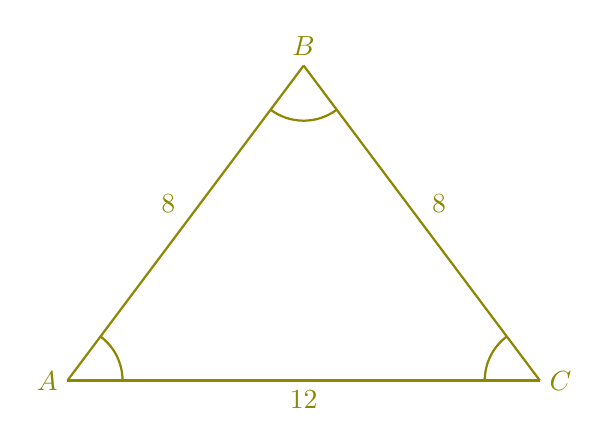
\begin{tikzpicture}
		%A
		\pgfmathsetmacro{\ax}{0}
		\pgfmathsetmacro{\ay}{0}
		%B
		\pgfmathsetmacro{\bx}{3}
		\pgfmathsetmacro{\by}{4}
		%C
		\pgfmathsetmacro{\cx}{6}
		\pgfmathsetmacro{\cy}{0}
		%arc radius
		\pgfmathsetmacro{\arclen}{0.7}
		%c
		\draw[color = olive, thick] (\ax,\ay) -- (\bx,\by) node[midway, anchor = south east] {$8$};
		%b
		\draw[color = olive, thick] (\ax,\ay) -- (\cx,\cy) node[midway, anchor = north] {$12$};
		%a
		\draw[color = olive, thick] (\bx,\by) -- (\cx,\cy) node[midway, anchor = south west] {$8$};
	%	Vinkel A		
		\draw[color = olive, thick] (\ax + \arclen,0) arc (0:53.13:\arclen) 
		node[midway, anchor = west] {};
	%	Vinkel B
		\draw[color = olive, thick] (2.58,3.44) arc (180 + 53.13:180 + 53.13 + 73.74:\arclen)
		 node[midway, anchor = south east] {};
	%	Vinkel C
		\draw[color = olive, thick] (\cx - \arclen,0) arc (180:180 - 53.13:\arclen)
		 node[midway, anchor = east] {};
		 %Nodes
		 \node[color = olive, anchor = east] at (\ax,\ay) {$A$};
		 \node[color = olive, anchor = south] at (\bx,\by) {$B$};
		 \node[color = olive, anchor = west] at (\cx,\cy) {$C$};
		\end{tikzpicture}
	\end{minipage}
\end{center}

\subsection*{Opgave 5 (med hjælpemidler)}
En trekant $\triangle ABC$ opfylder, at $\angle C = 29^\circ$, $a = 22$ og $b = 9$.
\begin{enumerate}[label=\roman*)]
	\item Bestem sidelængden $c$.
\end{enumerate}

\subsection*{Opgave 6 (med hjælpemidler)}
En trekant $\triangle ABC$ opfylder, at $\angle B = 70^\circ$, $a = 6$ og $c = 11$.
\begin{enumerate}[label=\roman*)	]
	\item Tegn en skitse af $\triangle ABC$. 
	\item Bestem de resterende sidelængder og vinkler i $\triangle ABC$ ved brug af både sinus- og 
	cosinusrelationerne
\end{enumerate}

\subsection*{Opgave 7 (med hjælpemidler)}
En trekant $\triangle ABC$ har $a = 20$, $b = 17$ og $\angle B = 112^\circ$.
\begin{enumerate}[label=\roman*)]
	\item Tegn en skitse af $\triangle ABC$.
	\item Bestem de resterende sidelængder og vinkler ved brug af sinus- og cosinusrelationerne. 
\end{enumerate}

